% theory_vs_reality.tex
\begin{frame}
  \onslide<1->{
	\frametitle{Kalman Filter Theory vs. Reality} 
	\framesubtitle{Kalman Assumption Recap}
}
\begin{itemize}
  \onslide<2->{
\item Kalman Assumptions
}
  \onslide<3->{
\begin{itemize}
\item All states linear are modeled correctly
\item Noise parameters are accurately known
\item Initial values are appropriate
\item Process and measurement noise are both Gaussian:  $w\sim\text{N}(0,Q)$, and $v\sim\text{N}(0,R)$
\item Process noise and measurement noise are uncorrelated
\item Measurements are taken at regularly scheduled intervals
\end{itemize} 
}
\end{itemize}
\end{frame}

\begin{frame}
  \onslide<1->{
	\frametitle{Kalman Filter Theory vs. Reality} 
	\framesubtitle{Other Potential Problems}
}
\begin{itemize}
  \onslide<2->{
\item  Continous filters useful for analytical work\\ (e.g., covariance analysis)
}
  \onslide<3->{
\item  But continous filters unrealistic in practice: Always some sort of discretization needed  
}
  \onslide<4->{
\item  Measurements almost never continuous 
}
  \onslide<5->{
\item  Discrete filters acceptable provided continuous estimates are not required 
}
  \onslide<5->{
\item  Suboptimality 
}
\end{itemize}
\end{frame}

\begin{frame}
  \onslide<1->{
	\frametitle{Kalman Filter Theory vs. Reality} 
	\framesubtitle{Sensor Selection}
}
\begin{itemize}
  \onslide<2->{
  \item How do you select appropriate sensors for the problem at hand?
}
  \onslide<3->{
  \item Some obvious general rules:
  \begin{itemize}
	\item The lower the sensor noise characteristics, the more accurate the estimates (narrow sensor noise variance)
}
  \onslide<4->{
    \item The more the merrier, i.e., the more sensors the better\\
	Greater number of lower quality sensors can outperform smaller number of higher quality ones (see kalcompare.m)
}
  \onslide<5->{
    \item Maximize the number of directly observable states
\end{itemize}
}
\end{itemize}
\end{frame}


\begin{frame}
  \onslide<1->{
	\frametitle{Kalman Filter Theory vs. Reality} 
	\framesubtitle{Sensor Selection}
}
\begin{itemize}
  \onslide<2->{
  \item Some less obvious general rules:
}
  \onslide<3->{
  \begin{itemize}
	\item Short-term / long-term complementarity (e.g, GPS vs. INS)
}
  \onslide<4->{
    \item Frequency response of sensor should match that of system
}
  \onslide<5->{
    \item Noise spectrum of sensor should be maximally disjoint from that of system
  \end{itemize}
}
\end{itemize}
\end{frame}

\begin{frame}
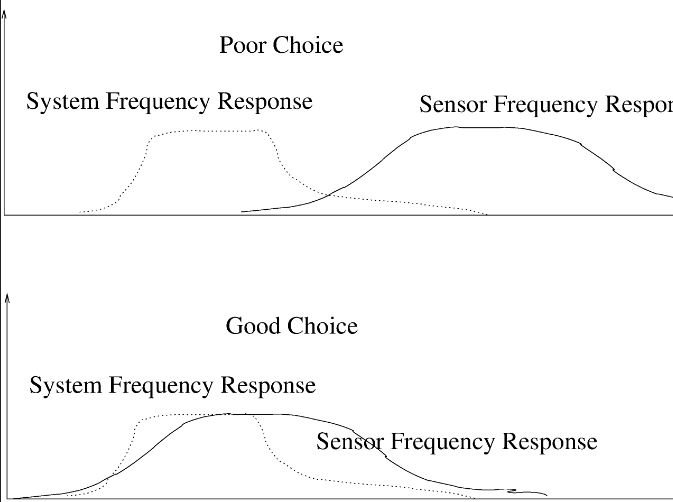
\includegraphics[scale=0.60]{day3_seg1_numerical/sensor_selection.jpg}
\end{frame}

\begin{frame}
  \onslide<1->{
	\frametitle{Kalman Filter Theory vs. Reality} 
	\framesubtitle{}
}
\begin{itemize}
  \onslide<2->{
  \item Choose sensors to match states.\\
E.g., consider the state model
\[
\begin{bmatrix}
\dot{x}_1\\
\dot{x}_2
\end{bmatrix}
= \begin{bmatrix}
0\\
0
\end{bmatrix}
\]
with the measurement model
\[
z = \begin{bmatrix} 1\;\; 0 \end{bmatrix}\begin{bmatrix}
x_1\\
x_2
\end{bmatrix}
+ v
\]
}
  \onslide<3->{
\item   Here $x_1$ is observable but $x_2$ is not, because there are no dynamic paths in $A=I$ flow infomation 
about $x_1$ into $x_2$
}
\end{itemize}
\end{frame}

\begin{frame}
  \onslide<1->{
	\frametitle{Kalman Filter Theory vs. Reality} 
	\framesubtitle{Sensor Selection}
}
\begin{itemize}
  \onslide<2->{
  \item Examine the $H$ matrix that you would use with this sensor!
}
  \onslide<3->{
  \item If it renders some states unobservable, then consider adding 
  additional sensors for those states, or replacing this sensor with one that is more favorable
}
\end{itemize}
\end{frame}
% day3_seg4_ins_challenges/observability.tex
\begin{frame}
  \onslide<1->{
	\frametitle{Observability} 
	\framesubtitle{}
}
\begin{itemize}
  \onslide<2->{
 \item Structural observability is concerned with how $H$ maps measurements into states
}
  \onslide<3->{
  \item Observability means there is a linear path from the measurements to states
}
  \onslide<4->{
  \item Structural observability determined by $\Phi$ and $H$:
}
  \onslide<5->{
\item  If $H$ is $1\times n$, where $n$ is the size of the state vector, then the state $x_0$ 
is said to be \textbf{observable }from $n$ scalar measurements $\set{z_0,\ldots,z_{n-1}}$ if the block matrix
\[
\begin{bmatrix}
H\trans&\Phi\trans H\trans & \cdots & (\Phi\trans)^{n-1}H\trans
\end{bmatrix}
\]
is of rank $n$

}
  \onslide<6->{
 \item Will making measurements as governed by $H$ actually enable us to estimate all of the states 
 in the state vector? 
}
 \end{itemize}
\end{frame}

\begin{frame}
  \onslide<1->{
	\frametitle{Observability} 
	\framesubtitle{Designing Observability into the Filter}
}
\begin{itemize}
  \onslide<2->{
  \item Observability challenge for filters is often a matter of choosing right kinds of sensors
}
  \onslide<3->{
  \item Choosing the right measurement scheduling
}
  \onslide<4->{
  \item Certain kinds of divergence can be the result of poor observability
}
  \onslide<5->{
\item   Example: Let $H=\left[1\;\;0\;\; 0\;\; 0\;\; 0\right]$, 
$\Phi=
\begin{bmatrix}
0&1&0&0&0\\
0&0&1&0&0\\
0&0&0&1&0\\
0&0&0&0&1\\
1& 2&3&4&5
\end{bmatrix}$
}
  \onslide<6->{
	\item What is the rank 
	of $\left[H\trans\;\;\Phi H\trans\;\;\Phi^2 H\trans\;\; \Phi^3 H\trans\;\;\Phi^4 H\trans\right]$?
}
\end{itemize}
\end{frame}


